\documentclass[10pt,a4paper]{article}
\usepackage[utf8]{inputenc}
\usepackage[french]{babel}
\usepackage[T1]{fontenc}
\usepackage{amsmath}
\usepackage{amsfonts}
\usepackage{amssymb}
\usepackage{graphicx}
\usepackage{caption}
\usepackage{subcaption}
\usepackage{geometry}
\geometry{hmargin=2.5cm,vmargin=1.cm}
\begin{document}
\section{Benchmark entre algo}

 \begin{figure}[ht]
 \centering
 	  \begin{subfigure}[b]{0.4\textwidth}
                 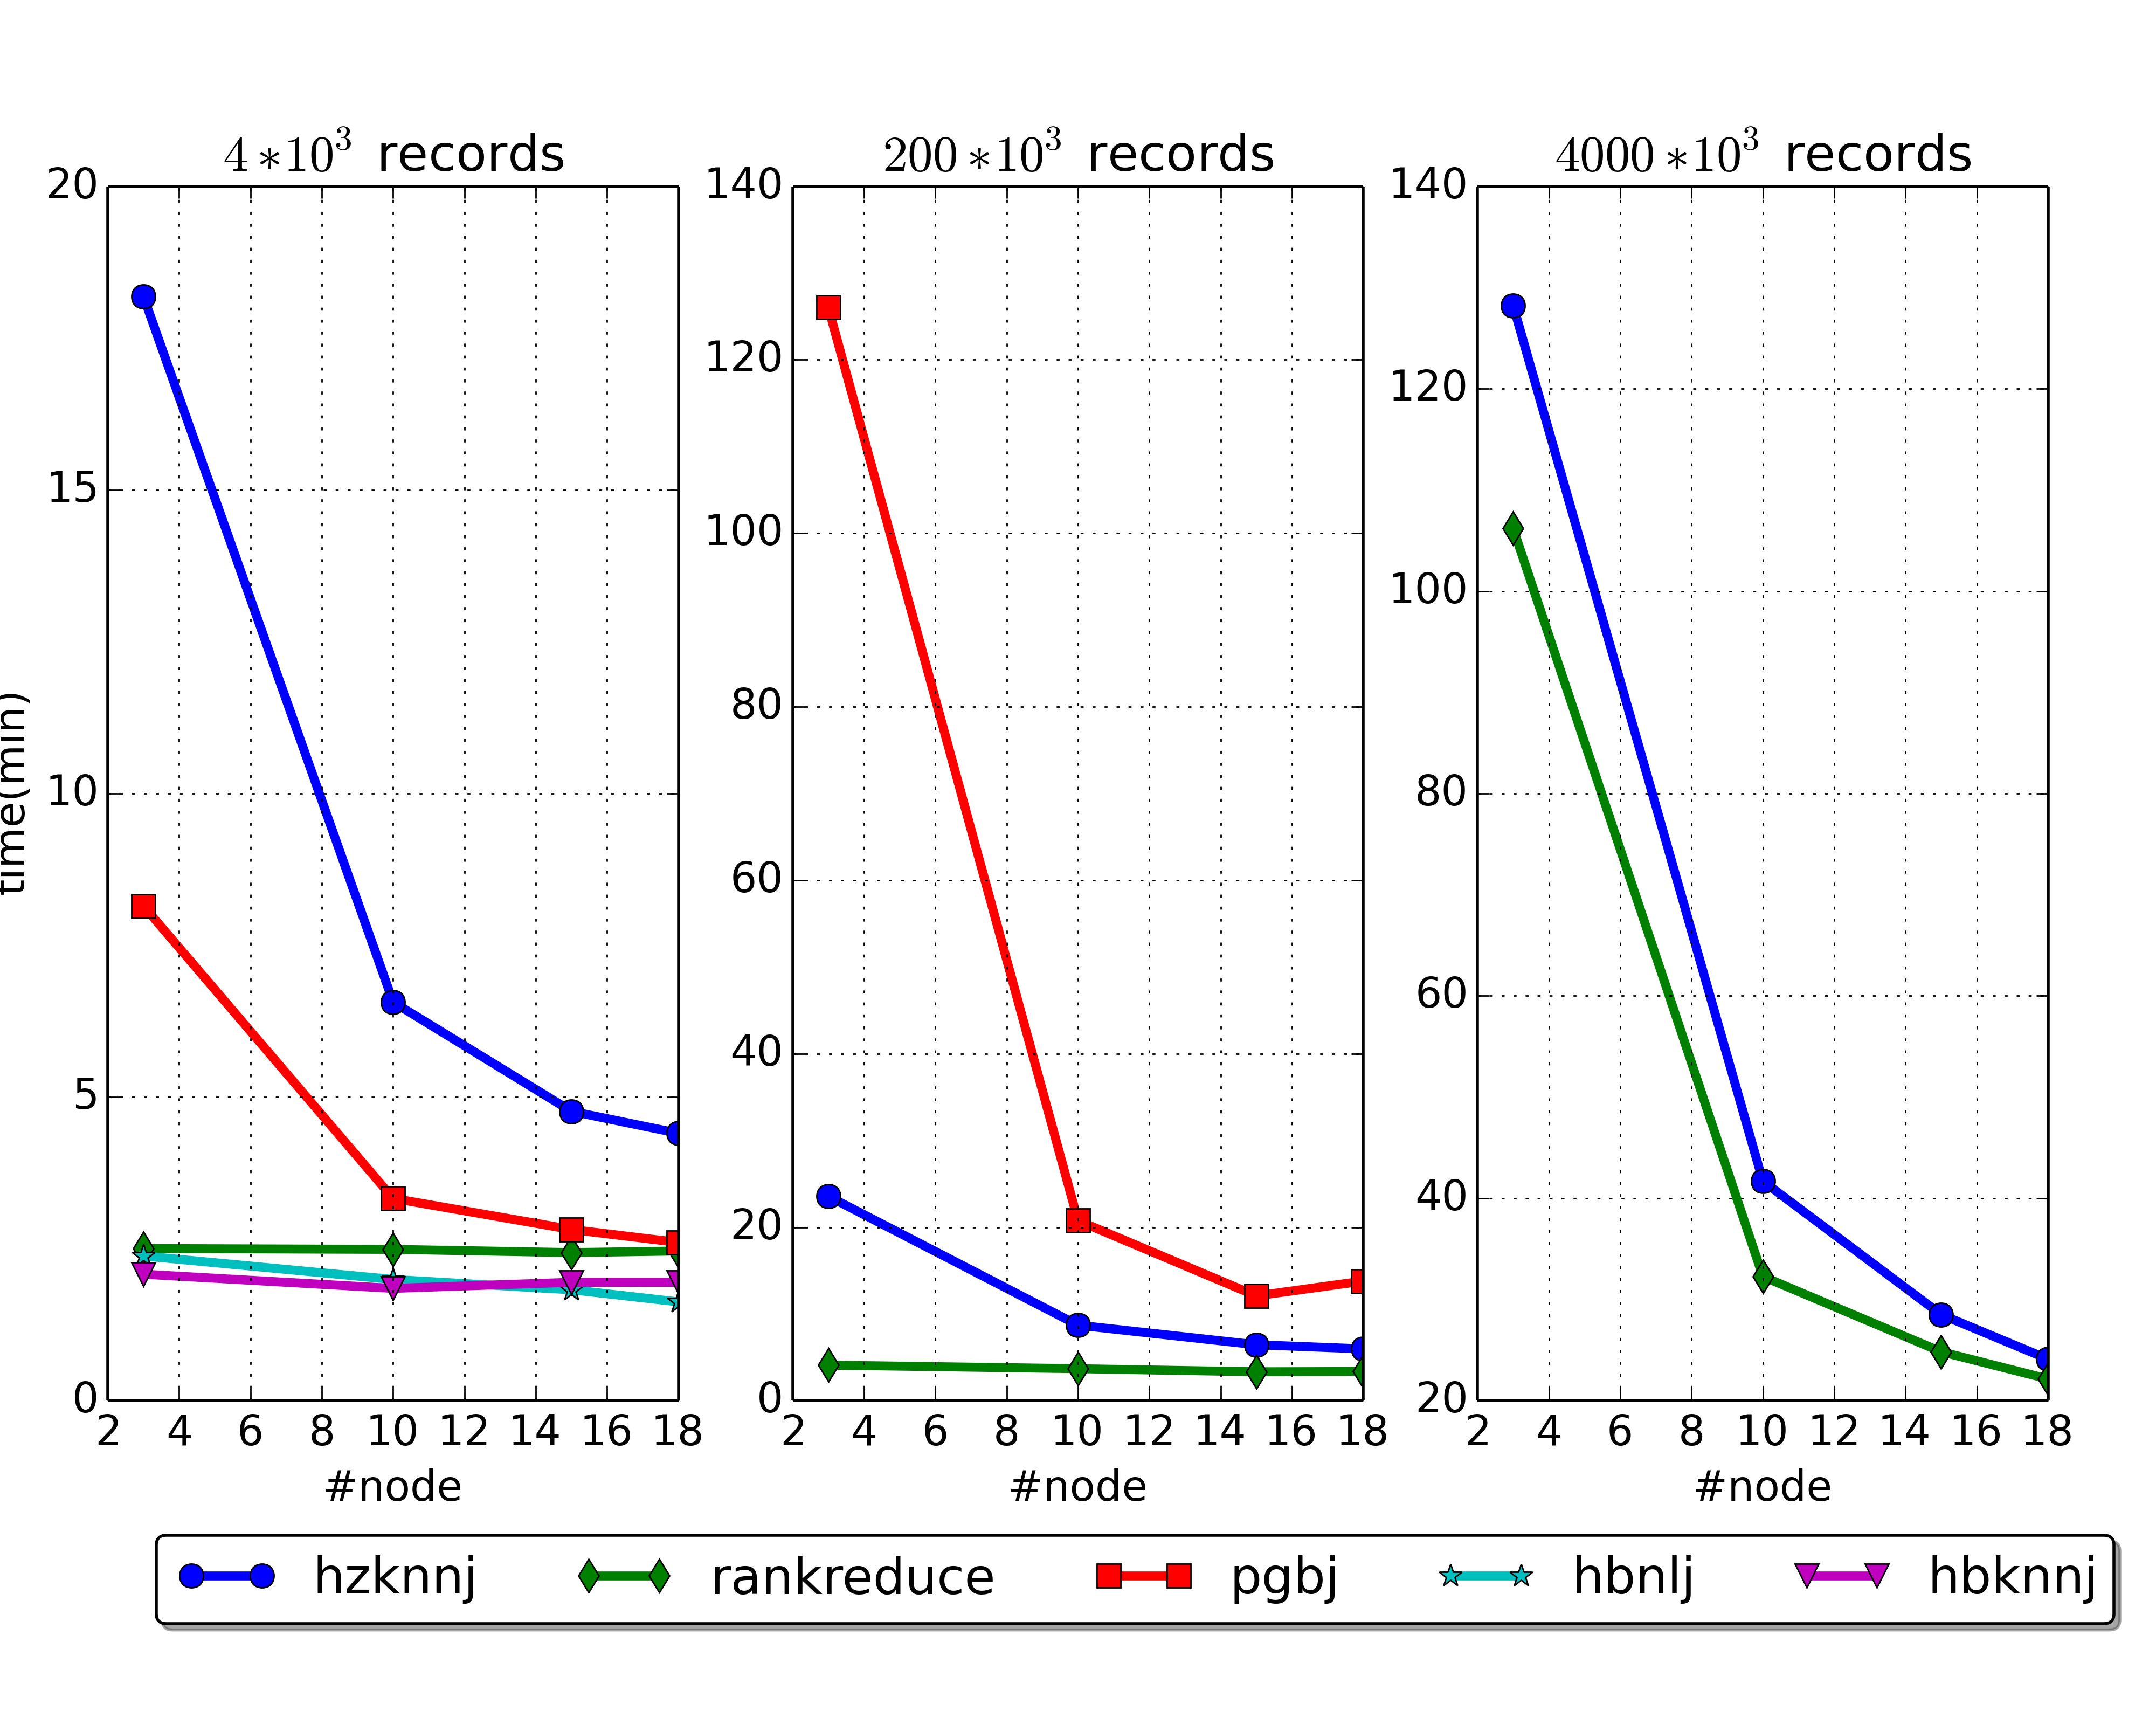
\includegraphics[width=\textwidth]{../graph/geo/nodes.png} 
                \caption{low dimension}
        \end{subfigure}%
        \begin{subfigure}[b]{0.4\textwidth}
                 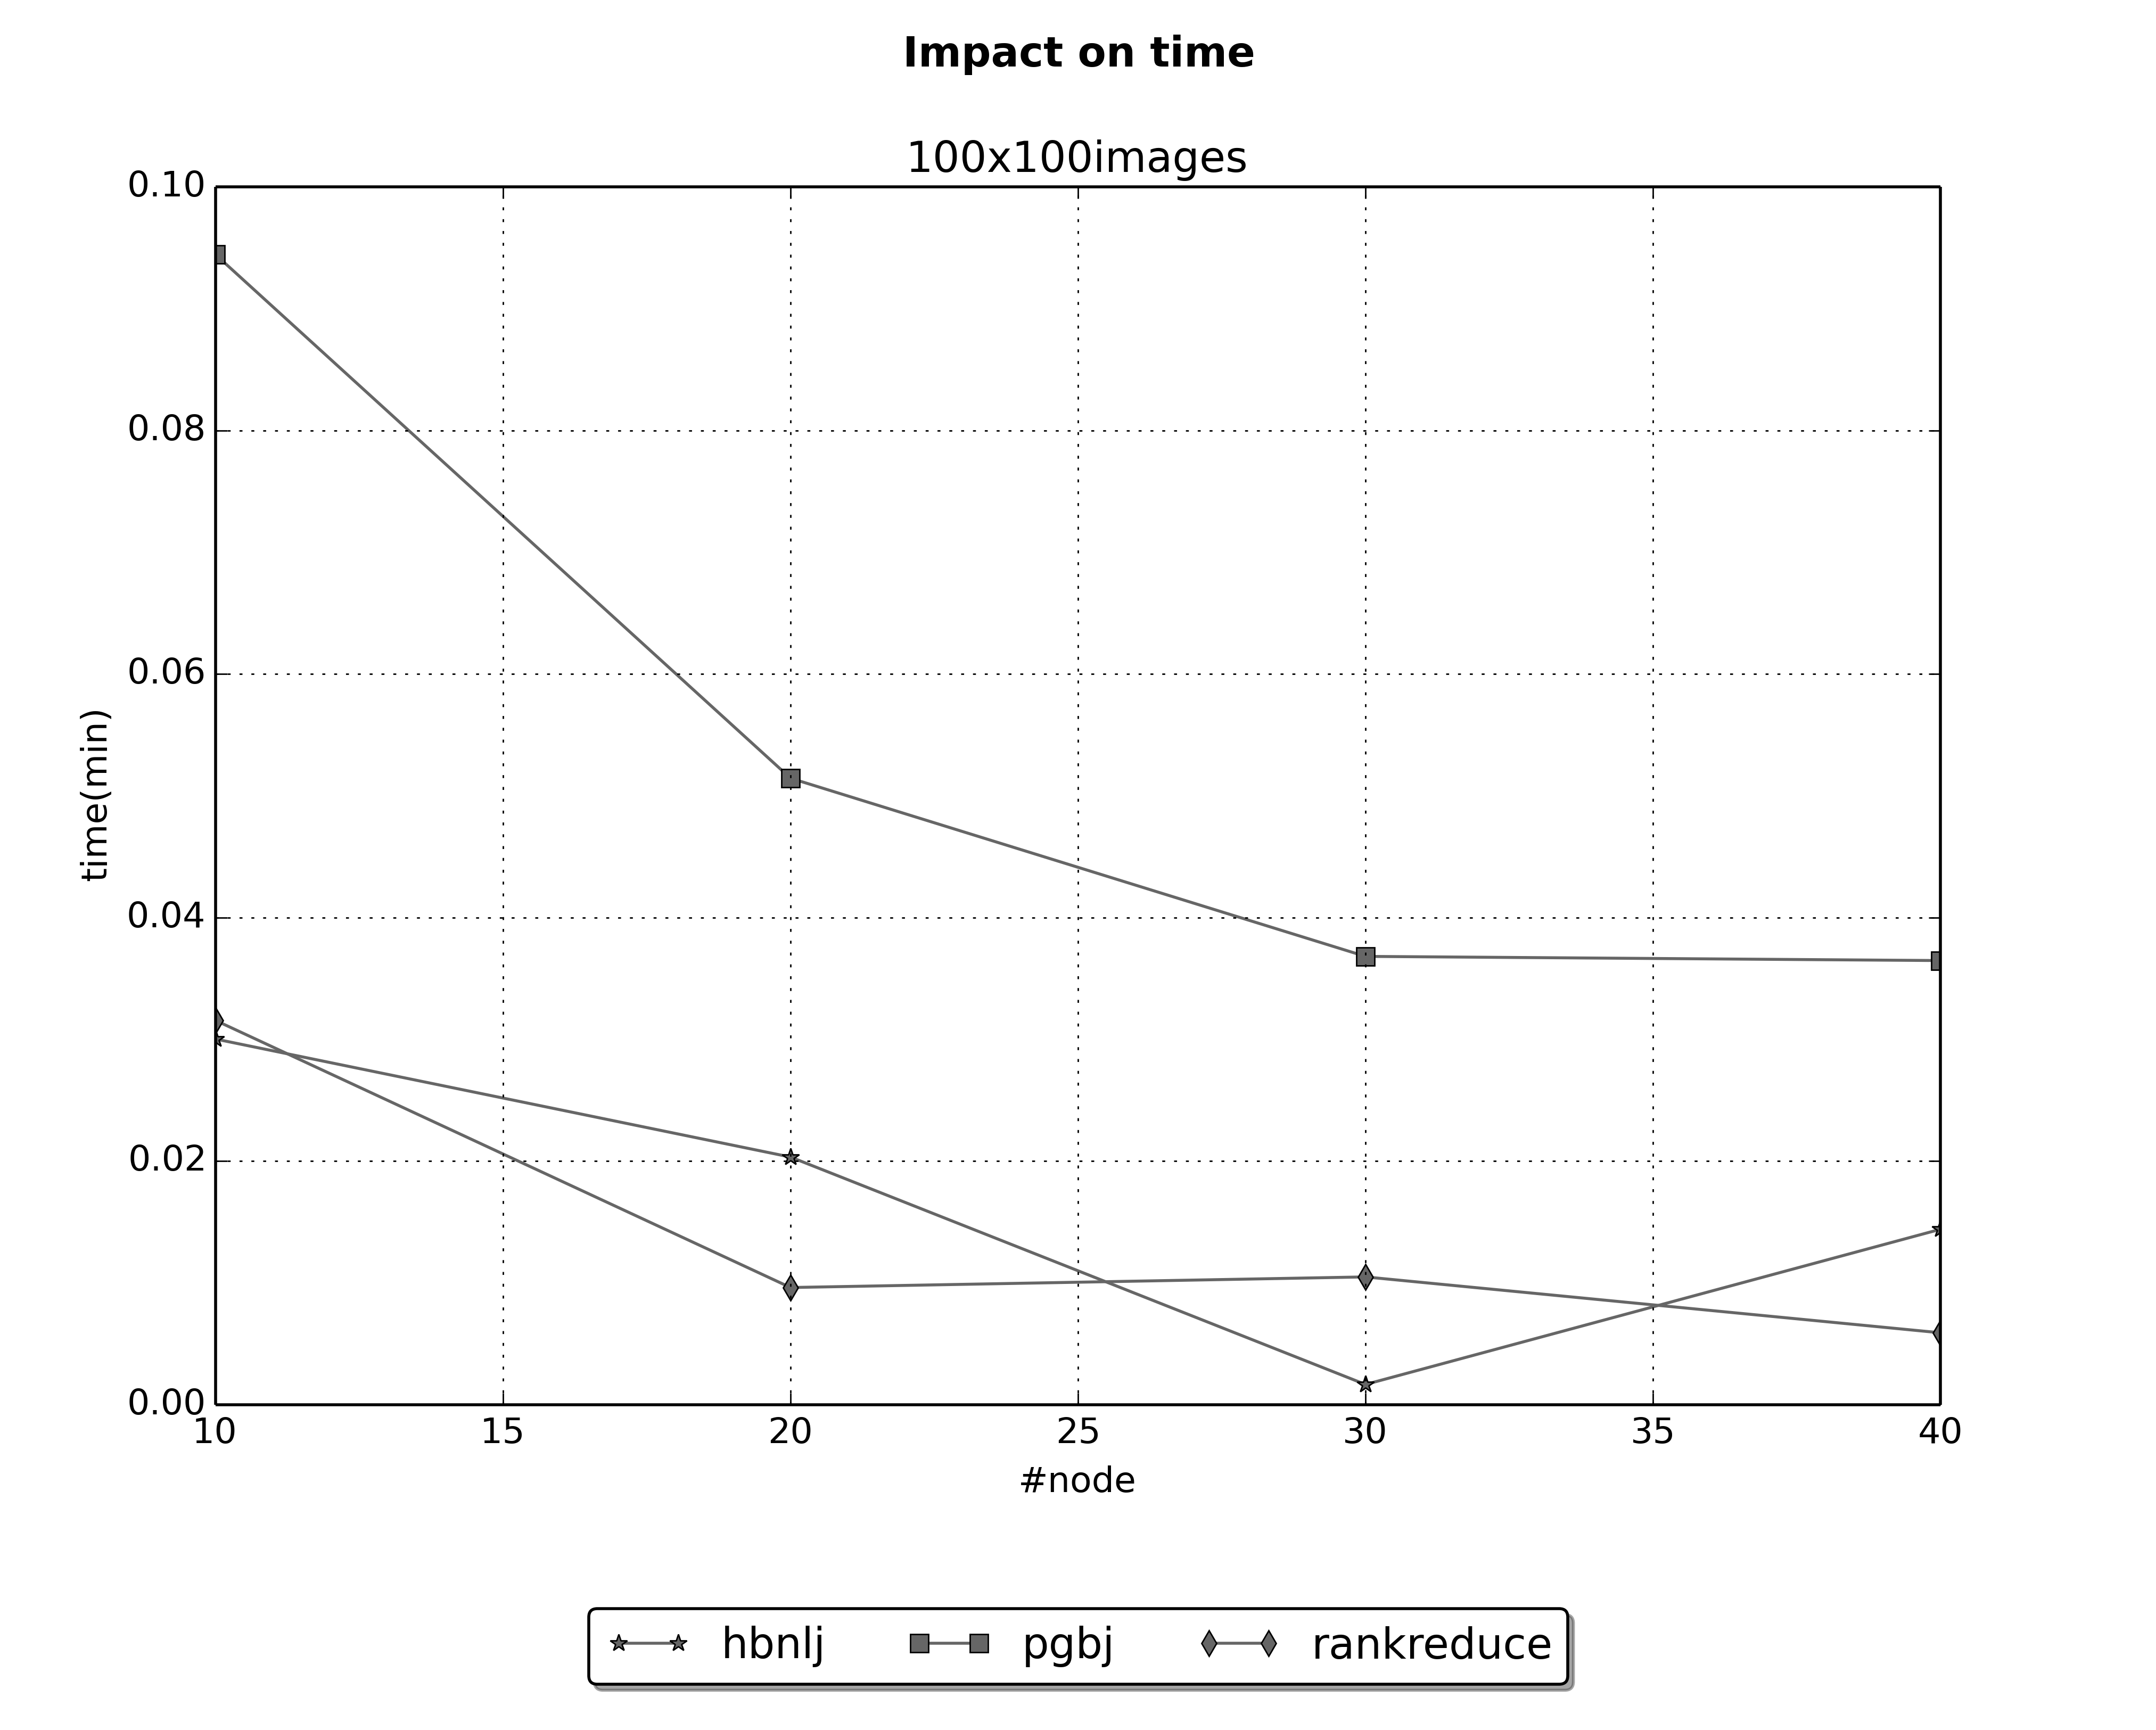
\includegraphics[width=\textwidth]{../graph/surf/nodes.png} 
                \caption{hight dimension}
        \end{subfigure}%
        \caption{Nodes}
  \end{figure}
  
  \begin{figure}[ht]
  \centering
 	  \begin{subfigure}[b]{0.4\textwidth}
                 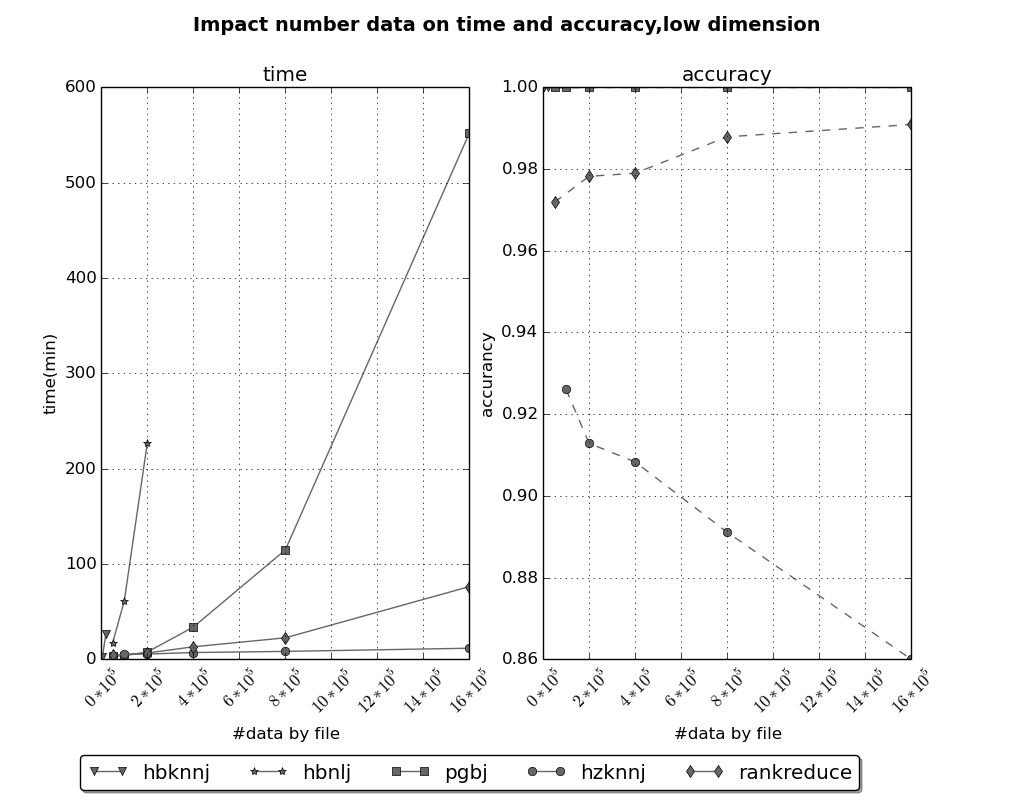
\includegraphics[width=\textwidth]{../graph/geo/time.png} 
                \caption{low dimension}
        \end{subfigure}%
        \begin{subfigure}[b]{0.4\textwidth}
                 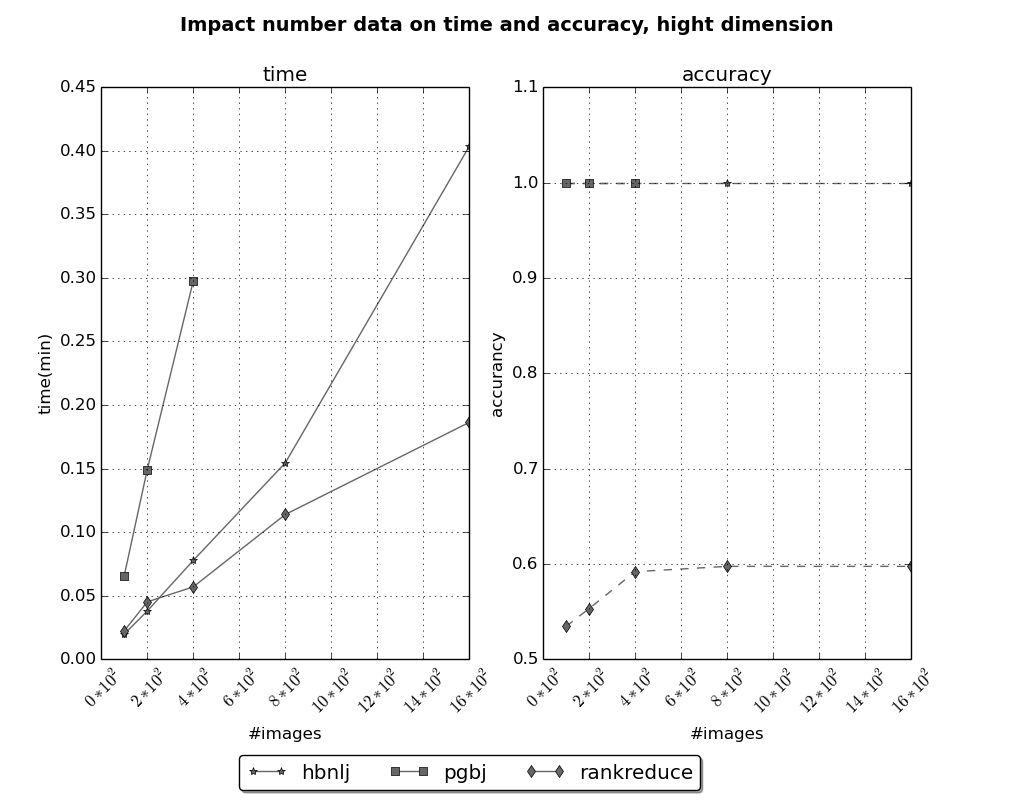
\includegraphics[width=\textwidth]{../graph/surf/time.png} 
                \caption{hight dimension}
        \end{subfigure}%
        \caption{K}
  \end{figure}
  
  \begin{figure}[ht]
  \centering
 	  \begin{subfigure}[b]{0.4\textwidth}
                 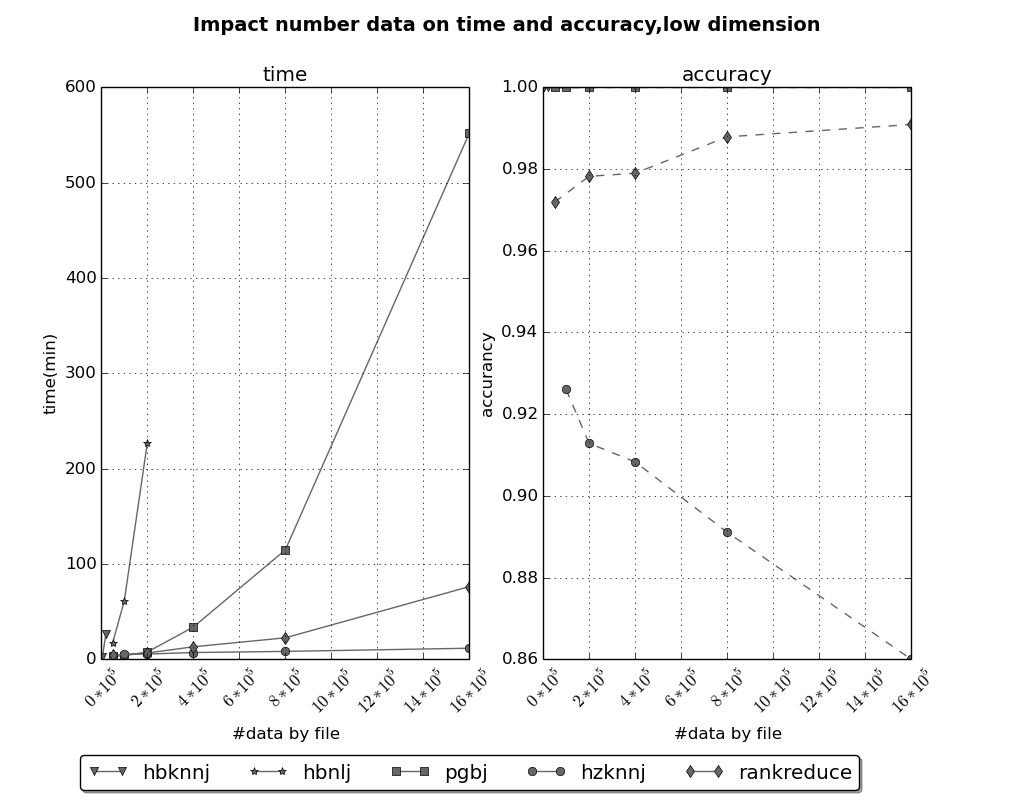
\includegraphics[width=\textwidth]{../graph/geo/time.png} 
                \caption{low dimension}
        \end{subfigure}%
        \begin{subfigure}[b]{0.4\textwidth}
                 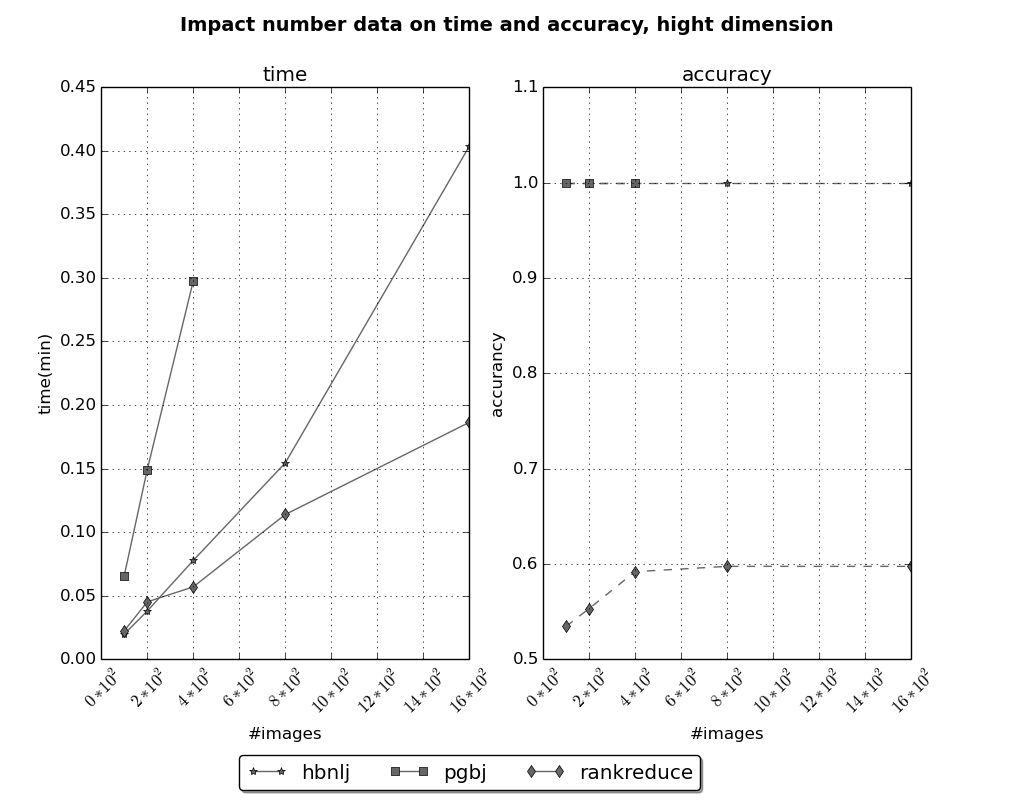
\includegraphics[width=\textwidth]{../graph/surf/time.png} 
                \caption{hight dimension}
        \end{subfigure}%
        \caption{time}
  \end{figure}
   \newpage

\end{document}